%%%%%%%%%%%%%%%%%%%%%%%%%%%%%%%%%%%%%%%%%%%%%%%%%%%%%%%%%%%%%%%%%%%%%%%%%%%%%%%%
\chapter{Machine Learning\label{chap:ML}}
%%%%%%%%%%%%%%%%%%%%%%%%%%%%%%%%%%%%%%%%%%%%%%%%%%%%%%%%%%%%%%%%%%%%%%%%%%%%%%%%

% 2) A feedforward neural network, as formally defined in the article concerning feedforward neural networks, whose parameters are collectively denoted θ\thetaθ. In backpropagation, the parameters of primary interest are wijkw_{ij}^kwijk​, the weight between node jjj in layer lkl_klk​ and node iii in layer lk−1l_{k-1}lk−1​, and bikb_i^kbik​, the bias for node iii in layer lkl_klk​. There are no connections between nodes in the same layer and layers are fully connected.
% 3) An error function, E(X,θ)E(X, \theta)E(X,θ), which defines the error between the desired output yi⃗\vec{y_i}yi
%  and the calculated output yi⃗^\hat{\vec{y_i}}yi​​^​ of the neural network on input xi⃗\vec{x_i}xi​​ for a set of input-output pairs (xi⃗,yi⃗)∈X\big(\vec{x_i}, \vec{y_i}\big) \in X(xi​​,yi​​)∈X and a particular value of the parameters θ\thetaθ.

\Gls{ML}, often described as a proper subset of \gls{AI}
\cite{Goodfellow-et-al-2016}, and is the field in computer science which deals
with the improvement of algorithms through experience and the use of data
\cite{Mitchell97}. Our daily lives exhibit wide applications of intelligent
software to automate routine labour, understand speech or images, assist in
diagnoses in medicine and support basic scientific research. This field as a
whole is relatively young, having been coined in 1959 by Arthur Samuel
\cite{5392560}, however little progress in reaching human-comparable learning
was achieved until the advent of deep learning, termed by Rina Dechter in 1986
\cite{Rina1986}. Even then, human-like recognition of real-world images was not
achieved until ImageNet was created in 2009 \cite{5206848}, which is often
considered as the catalyst for the AI boom of the 21st century
\cite{hardy_2016}.

\begin{figure}[htp!]
    \centering
    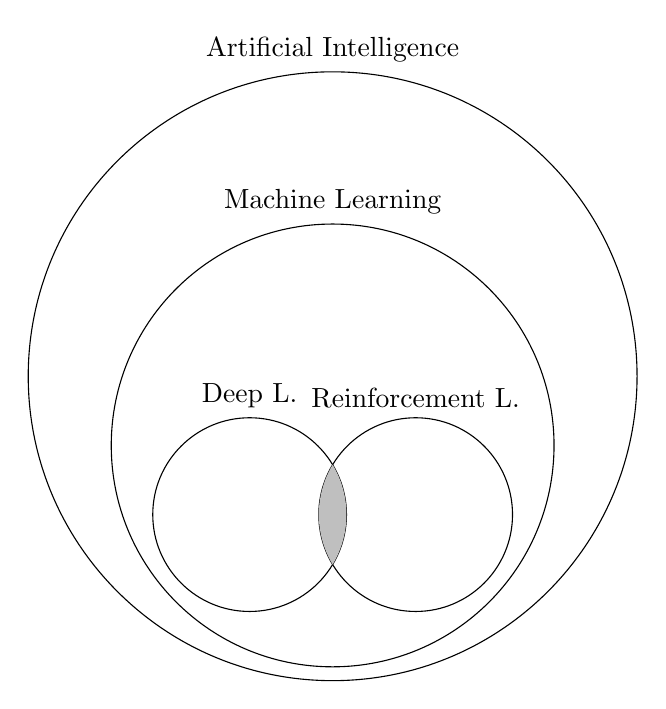
\begin{tikzpicture}

    % Circle with label
    \node[draw,
        circle,
        minimum size =22em,
        label=Artificial Intelligence] (ai_circ) at (0,0){};

    % Circle with label
    \node[draw,
        circle,
        minimum size =16em,
        label=Machine Learning] (ml_circ) at (0,-2.5em){};

    % Circle with label
    \node[draw,
        circle,
        minimum size =7em,
        label=Deep L.] (dl_circ) at (-3em,-5em){};

    \node[draw,
        circle,
        minimum size =7em,
        label=Reinforcement L.] (rl_circ) at (3em,-5em){};


    % Intersection
    \begin{scope}
        \clip (-3em,-5em) circle(3.5em);
        \clip (3em,-5em) circle(3.5em);
        \fill[gray!50](3em,-5em) circle(3.5em);
    \end{scope}

\end{tikzpicture}
    \captionsetup{format=hang} % hanging captions
    \caption{
        The relationship between the fields of Artificial Intelligence,
        Machine Learning, Deep Learning and Reinforcement Learning with some
        arbitrary example provided per field.
    }
    \label{fig:al-ml-dl}
\end{figure}


\newpage


\section{Machine Learning Basics}
%%%%%%%%%%%%%%%%%%%%%%%%%%%%%%%%%%%%%%%%%%%%%%%%%%%%%%%%%%%%%%%%%%%%%%%%%%%%%%%%
This section aims at a providing a non-exhaustive coverage of the basics of
machine learning can can be applied to all machine learning algorithms. This
section starts by defining what is meant when it is said that an algorithm
``learns". The types of datasets that may be encountered in the application of
these learning algorithms are then briefly covered to provide insight into the
potential applications which are not covered in this review. The distinction is
then made between the goal of fitting training data and the goal of finding
patterns that generalize to new data. This section then covers a very common
concept in machine learning: \textit{hyperparameters}, which are
\textit{settings} of a learning algorithm which must be determined outside the
learning algorithm itself.

\subsection{Learning algorithms}
%%%%%%%%%%%%%%%%%%%%%%%%%%%%%%%%%%%%%%%%%%%%%%%%%%%%%%%%%%%%%%%%%%%%%%%%%%%%%%%%
Generally speaking, a machine learning algorithm is a procedure for learning
from data.However correct this definition is, it provides little insight into
the relevant concepts in the field. A more succint definition is provided by
Mitchell \cite{Mitchell97LearningAlgorithm}:
\begin{quotation}
    \textit{
        A computer program is said to learn from experience $E$ with respect to
        some class of tasks $T$ and a performance measure $P$, if its
        performance at tasks in $T$, as measured by $P$, improves with
        experience $E$.
    }
\end{quotation}
This definition introduces the general entities which are present during all
machine learning tasks. The entities will not be formally defined in the
following sections as it is far outside the scope of this literature, and is
philosophical in nature. This section will instead cover examples of each which
will provide practical insight on which the reader can build their knowledge.

\subsubsection{The Task, $T$}
%%%%%%%%%%%%%%%%%%%%%%%%%%%%%%%%%%%%%%%%%%%%%%%%%%%%%%%%%%%%%%%%%%%%%%%%%%%%%%%%
There exists a plethora of tasks which humanity has applied learning algorithms
to during the timeline of the field. It is common for \gls{ML} practitioners to
originate from domains outside that of computer science, in order to access the
feasibility of existing algorithms in their domain. There is however a question
that often presents itself to specialists in their respective fields when they
consider applying \gls{ML} to the existing problems in their field. Why should a
specialist opt for solving problems with \gls{ML} that have been solved using
tried and true techniques in their domain of expertise? Goodfellow et al.
\cite{Goodfellow-et-al-2016} provide an insightful response to this:

\begin{quotation}
    \textit{
        Machine learning enables us to tackle tasks that are too difficult to
        solve with fixed programs written and designed by human beings. From a
        scientific and philosophical point of view, machine learning is
        interesting because developing our understanding of it entails
        developing our understanding of the principles that underlie
        intelligence.
    }
\end{quotation}
An example of a field which has undergone dramatic changes in a short period of
time, with the advent of \gls{DL} and modern hardware, is \gls{CV}. Mahony et.
al. discuss this in their paper with a focus on comparing \gls{DL} and \gls{CV}
\cite{Mahony-et-al-2020}. Their paper concludes that many \gls{CV} techniques
invented in the 20 years preceding the paper have become irrelevant as a result
of \gls{DL}. However, they emphasise on the importance of the knowledge
established in those 20 years, arguing that \textit{``knowledge is never
obsolete"}, as it provides specialists with more tools and intuition when
addressing problems. Some typical applications of \gls{CV} are detailed and
although these may be outperformed by \gls{DL}, relying on \gls{DL} in some
cases is overkill. They also point out some hybrid approaches between \gls{DL}
and \gls{CV} which synergize, saying that \gls{CV} provides improved performance
in \gls{DL} by reducing training time. This emphasises that specialists should
not expect an end-all solution from \gls{ML} in addressing their domain-specific
problems, but rather as mentioned by Goodfellow et al., strive for a better
understanding of the principles that underlie intelligence, and by extension,
those that underlie the practitioners domain-specific problems.

\begin{itemize}
    \item \textbf{Classification}: In this task, the learning algorithm is
    expected to produce a function $f: \mathbb{R^n}\rightarrow
    \{1,...,k\}$. When $y=f(\mathbf{x})$, the model assigns a provided
    input, $\mathbf{x}$ to a category identified by numeric code $y$. An
    example of this would be the mapping of a grayscale image,
    $\mathbf{x}\in\mathbb{R}^2$ to a value corresponding to a numerical
    encoding $f:\mathbb{R}^n\rightarrow\{\textrm{Cat},\;\textrm{Dog}\}$.
    \item \textbf{Classification with missing inputs}: Classification becomes
    more challenging when the input measurements to the model are not
    guaranteed to always be the same. In this situation the algorithm must
    learn the set of all function mappings arising from the possible
    combinations of input vectors that arise from missing subsets of
    inputs in $\mathbf{x}$. An example of this would be the classification
    of a diagnosis in medicine, as depending on the invasiveness of
    certain procedures, different subsets of measurements are available.
    \item \textbf{Regression}: In this task, the learning algorithm is expected
    to predict a continuous numerical value for a given input. This is
    done by learning a function $f: \mathbb{R}^n\rightarrow\mathbb{R}$.
    the formulation is similar to that of classification, except for the
    output format. An example of this would be learning of a function to
    predict the expected returns for a given investment given the state of
    the market, as is common is algorithmic trading.
    \item \textbf{Transcription}: This type of task involves the learning
    algorithm observing a relatively unstructured input and transcribing
    it into some discrete textual form. An example of this is the
    transcription of an audio waveform containing speech into text.
    \item \textbf{Machine translation}: In machine translation, the already
    structured input is mapped into a different language. This is common
    in the field of \gls{NLP}, where languages are translated between, for
    example English and French. This however is not limited to natural
    languages but can also be applied to programming languages for
    example.
    \item \textbf{Structured output}: This task entails those where the output
    is a vector or a data structure which details important relationships
    between the contained elements. This task subsumes the prior two of
    transcription and machine translation. An example of this would be the
    parsing of grammatical structure of a natural language sentence,
    addressed in \gls{NLP} and demonstrated by Collobert
    \cite{pmlr-v15-collobert11a}.
    \item \textbf{Anomaly detection}: In this task, a learning algorithm learns
    to sift through a set of events and classify events that are anomalous
    in nature. These algorithms have been applied to credit card companies
    in detection of fraud \cite{DBLP:journals/corr/abs-2108-10005}, and in
    safety in the aviation industry \cite{Janakiraman2016, Basora2019}.
    \item \textbf{Synthesis and sampling}: In this task, learning algorithms
    generate \textbf{new} examples which appear to be drawn from the same
    underlying distribution as, but are not present in the training data.
    A recent example around which a lot of research is being done is the
    \gls{GPT-3} which is able to produce human-like text, given prompts as
    input \cite{DBLP:journals/corr/abs-2005-14165}.
    \item \textbf{Imputation of missing values}: In this task, the learning
    algorithm is given some input $x\in\mathbb{R}$ with some elements
    $x_i$ missing. The algorithm must then make predictions for the
    missing values. Emmanuel et. al. discuss the latest methods in
    \gls{ML} that address this task~\cite{Emmanuel2021}.
    \item \textbf{Denoising}: In this learning task, the machine learning
    algorithm learns to generate a clean example $\mathbf{x}\in\mathbb{R}^n$
    from a corrupted sample $\tilde{\mathbf{x}}\in\mathbb{R}^n$. Generally
    speaking the learner is predicting the probability distribution
    $p(\mathbf{x}|\tilde{\mathbf{x}})$.
    \item \textbf{Density estimation} or \textbf{probability mass function estimation}
    involves the task task of learning a function $p_\text{model}:\mathbb{R}^n\rightarrow{}\mathbb{R}$,
    where $p_\text{model}(\mathbf{x})$ is interpreted as a probability distribution function
    from which $\mathbf{x}$ was drawn. Effectively the algorithm learns the
    structure of the data that it has been provided with. Most of the
    aforementioned tasks involve learning this distribution function, at least
    implicitly. For example for the missing value imputation task, if $x_i$ is
    missing, and all other values $x_{-i}$ are given, then the algorithm learns
    the distribution $p(x_i|\mathbf{x}_{-i})$ which involves $p(\mathbf{x})$
    implicitly.
\end{itemize}
%An ongoing trend in society is the augmentation of responsibility in intelligent
%algorithms through autonomy, evident by the advent of semi-autonomous cars,
%autonomous cyber-security \cite{Taeihagh2019}, autonomous industrial site
%inspection\footnote{\url{https://newsroom.ibm.com/Boston-Dynamics-and-IBM-Join-Forces-to-Bring-Mobile-Edge-Analytics-to-Industrial-Operations}},
%and autonomous supply-chain
%management\footnote{\url{https://www.forbes.com/sites/stevebanker/2021/04/01/amazon-supply-chain-innovation-continues/}},
%to name a few.

%This section reviews the current ongoing research in the field of machine
%learning as a whole. First the main categories:

\subsubsection{The Performance, $P$\label{sec:ML-performance}}
%%%%%%%%%%%%%%%%%%%%%%%%%%%%%%%%%%%%%%%%%%%%%%%%%%%%%%%%%%%%%%%%%%%%%%%%%%%%%%%%
In order to access the performance of our learning algorithm in task $T$,
we must have some quantitative measure of performance $P$ with which we steer
the algorithm towards the desired behaviour. $T$ and $P$ in this way are
coupled, and must $P$ must be chosen according to $T$. In this way it can be
unclear to the \gls{ML} practitioner what $P$ should be chosen.

Firstly, it is worth considering the true goal of the learning algorithm. We
wish for it to train according to some dataset such that it can generalize to
inputs that it has never seen before. After all, there is little worth in a
classification algorithm recognizing cats and dogs with 90\% accuracy on its
training dataset, if it performs with 20\% accuracy on an unseen \textbf{test}
dataset. This previously mentioned scenario is known as \textit{overfitting} and
is discussed in its own section later in the chapter. For this reason, the first
requirement on managing our dataset is presented, there must be some
\textbf{train-test split}. This is further complicated by the
\textbf{validation} dataset which is discussed later in the chapter.

Given that the input-output pair is $\{\mathbf{x}_i, \mathbf{y}_i\}$,
$\mathbf{y}_i$ is commonly referred to as the \textit{ground truth}, and
$\hat{\mathbf{f}}(\mathbf{x}_i)=\hat{\mathbf{y}}_i$ are referred to as the
\textit{predictor} and \textit{predicted output} respectively. The performance
in the form of a loss function $L$ is then some function of $\mathbf{y}_i$ and
$\hat{\mathbf{y}}_i$, therefore $L(\hat{\mathbf{y}}_i, \mathbf{y}_i)$.

\gls{ML} often borrows from \textit{approximation theory} vector norm notation
($\ell(\cdot)_p=||\cdot||_p$) to simplify notation in performance metrics. See
\autoref{appendix:vector_norms} for the expressions of vector norms.

\textbf{Regression loss functions}
\begin{itemize}
    \item \textbf{\Gls{MSE}} is the average of the squared differences between
    predictions and the ground truth. It is only concerned with the average
    magnitude of errors irrespective of their direction. Due to the squaring,
    predictions which have greater errors are more heavily penalized. A
    beneficial mathematical property of \gls{MSE} is that gradients can be
    easily calculated.
    \begin{equation}
        L_\text{MSE} = \frac{1}{N}\sum_{i=1}^{N}||\hat{\mathbf{y}}_i-\mathbf{y}_i||^2_2
    \end{equation}
    \item \textbf{L2 error} is the average of the differences between
    predictions and the ground truth. It is the same as \gls{MSE} but without
    the squaring. Like \gls{MSE}, the gradient can be easily calculated.
    \begin{equation}
        L_\text{L2E} = \frac{1}{N}\sum_{i=1}^{N}||\hat{\mathbf{y}}_i-\mathbf{y}_i||_2
    \end{equation}
    \item \textbf{\Gls{MAE}} or \textbf{L1 loss} is the average of the sum of
    absolute differences between predictions and the ground truth. This measure
    is similar to \gls{MSE} in that it considers the magnitude of the errors and
    ignores their direction. However, \gls{MAE} is more difficult to compute
    gradients for, requiring linear programming. \gls{MAE} is also more
    resilient to large error values as a result of outliers, as it does not make
    use of a square.
    \begin{equation}
        L_\text{MAE} = \frac{1}{N}\sum_{i=1}^{N}||\hat{\mathbf{y}}_i-\mathbf{y}_i||_1
    \end{equation}
    \item \textbf{\Gls{MBE}}
    \begin{equation}
        L_\text{MBE} = \frac{1}{N}\sum_{i=1}^{N}(\hat{\mathbf{y}}_i-\mathbf{y}_i)
    \end{equation}
    \item \textbf{\Gls{MSLE}}
    \begin{equation}
        \begin{aligned}
            L_\text{MSLE} &= \frac{1}{N}\sum_{i=1}^{N}(\log{(y_i+1)} - \log{(\hat{\mathbf{y}}_i+1)})^2 \\
            &= \frac{1}{N}\sum_{i=1}^{N}2\log(\frac{y_i+1}{\hat{\mathbf{y}}_i+1})
        \end{aligned}
    \end{equation}
    \item \textbf{Cosine Proximity}
    \begin{equation}
        L_\text{cos} = -\frac{\mathbf{y}_i\cdot{}\hat{\mathbf{y}}_i}{||\mathbf{y}_i||_2\cdot{}||\hat{\mathbf{y}}_i||_2}
    \end{equation}
\end{itemize}


\textbf{Binary classification loss functions}
\begin{itemize}
    \item Binary cross-entropy
    \begin{equation}
        L=-\sum_{i=1}^N\bigg(y_i\log(\hat{\mathbf{y}}_i)+(1-y_i)\log(1-\hat{\mathbf{y}}_i)\bigg)\label{eq:equation}
    \end{equation}
    \item Hinge loss
    \begin{equation}

    \end{equation}
    \item Squared hinge loss
\end{itemize}

\textbf{Multi-class classification loss functions}
\begin{itemize}
    \item Multi-class cross-entropy
    \begin{equation}
        L_{CE}=-\sum_{i=1}^N\sum_{j=1}^{M}y_{ij}\log(\hat{f}_j(\mathbf{x}_i))
    \end{equation}
    \item Hinge loss
    \item Squared hinge loss
\end{itemize}


\begin{itemize}
\end{itemize}
%With the
%In the case of classification, most metrics are derived from the confusion
%matric

\subsubsection{The Experience, $E$\label{sec:ML-experience}}
%%%%%%%%%%%%%%%%%%%%%%%%%%%%%%%%%%%%%%%%%%%%%%%%%%%%%%%%%%%%%%%%%%%%%%%%%%%%%%%%
Tasks provided to machine learning algorithms have different formulations based
on the experience made available. Learning algorithms can be broadly categorized
by the kind of experience that the algorithm has access to during learning, from
which it is generally expected to learn some pattern of interest.

\begin{itemize}
    \item \textbf{Supervised learning} algorithms experience a dataset
    containing features (input) and labels (expected output), and are expected
    to learn a function mapping between the two. These algorithms can be further
    divided into two categories. \textbf{Classification algorithms} learn a
    mapping from an input to a discrete class label output. \textbf{Regression
    algorithms} learn a mapping from an input to a continuous value output.

%    example input-output pairs, otherwise referred to as the labelled training
%    data consisting of a set of training examples. The trained \textit{model} is
%    then provided an unseen $x$ for which it must estimate $y$ based on its
%    experience. Supervised models are further grouped into two subcategories,
%    classification and regression. \textbf{Classification} is the task of
%    mapping $x$ to a discrete output variable $y$ which determines the predicted
%    class based on the $x$. A simple example of this would be a $y$ in
%    $\mathbb{R}^2$ which determines whether the input image was a \textit{cat}
%    or a \textit{dog}. \textbf{Regression} is task of mapping $x$ onto a
%    continuous output variable $y$ which determines the value of some variable
%    of interest. An example of this would be the task of learning an
%    approximator to the function: $f(x)=x^2$.
    % Dimensionality reduction \cite{vogelstein2021supervised}

    \item \textbf{Unsupervised learning} algorithms experience a dataset
    containing only features and learn some useful properties of the structure
    of the dataset. This form of learning often addresses recognition problems
    in \textit{association} \& \textit{clustering} \cite{barlow1999ul}.

    \item \textbf{Semi-supervised} is a middle ground between supervised
    learning (in which all training data is labelled) and unsupervised learning
    (in which no label data is provided)~\cite{books/mit/06/CSZ2006}. Some
    example applications of this paradigm are dimensionality reduction
    ~\cite{Zhang2007}, clustering \cite{Bair2013}, and anomaly detection
    \cite{DBLP:journals/corr/abs-1805-06725}.

    \item \textbf{Reinforcement learning} are learning algorithms which rely
    exclusively on a series of reinforcements from its environment. These
    reinforcements can be positive (rewards) or negative (punishments). This
    category is discussed further in \autoref{ssec:RL}.
\end{itemize}

\subsection{Capacity, Overfitting and Underfitting}
%%%%%%%%%%%%%%%%%%%%%%%%%%%%%%%%%%%%%%%%%%%%%%%%%%%%%%%%%%%%%%%%%%%%%%%%%%%%%%%%
The primary objective in \gls{ML} is to find a model which performs well on
previously \textit{unseen data}, which has not been used during the training or
fitting of a model. This ability of the learning algorithm is referred to as the
\textit{generalisation}.

Typically the learning algorithm is trained according to a set of
\textit{training data} with which we aim at reducing the learners
\textbf{training error}. Due to this data having been directly used to optimise
the moding during training, we cannot expect this error to be representative of
the \textbf{generalisation error}. In order to derive an estimate of the
generalisation error, we separate part of the initial data set into training and
\textbf{test data}, from which the \textbf{test error} is derived. Given some
assumptions about the \textbf{data-generating process}, it can be said that the
test error is equal to the expected generalisation error of the mode.

An important concept in \gls{ML} is the \textit{capacity} of the model. This is
defined informally as \textit{``a model’s [...] ability to fit a wide
variety of functions"}~\cite[p.~111-112]{Goodfellow-et-al-2016}.

\begin{figure}[htp]
    \centering
    % MIT License
%
% Copyright (c) 2021 Geoffrey H. Garrett
%
% Permission is hereby granted, free of charge, to any person obtaining a copy
% of this software and associated documentation files (the "Software"), to deal
% in the Software without restriction, including without limitation the rights
% to use, copy, modify, merge, publish, distribute, sublicense, and/or sell
% copies of the Software, and to permit persons to whom the Software is
% furnished to do so, subject to the following conditions:
%
% The above copyright notice and this permission notice shall be included in all
% copies or substantial portions of the Software.
%
% THE SOFTWARE IS PROVIDED "AS IS", WITHOUT WARRANTY OF ANY KIND, EXPRESS OR
% IMPLIED, INCLUDING BUT NOT LIMITED TO THE WARRANTIES OF MERCHANTABILITY,
% FITNESS FOR A PARTICULAR PURPOSE AND NONINFRINGEMENT. IN NO EVENT SHALL THE
% AUTHORS OR COPYRIGHT HOLDERS BE LIABLE FOR ANY CLAIM, DAMAGES OR OTHER
% LIABILITY, WHETHER IN AN ACTION OF CONTRACT, TORT OR OTHERWISE, ARISING FROM,
% OUT OF OR IN CONNECTION WITH THE SOFTWARE OR THE USE OR OTHER DEALINGS IN THE
% SOFTWARE.

%%%%%%%%%%%%%%%%%%%%%%%%%%%%%%%%%%%%%%%%%%%%%%%%%%%%%%%%%%%%%%%%%%%%%%%%%%%%%%%
% ACKNOWLEDGEMENTS
%%%%%%%%%%%%%%%%%%%%%%%%%%%%%%%%%%%%%%%%%%%%%%%%%%%%%%%%%%%%%%%%%%%%%%%%%%%%%%%
% Design and implementation of this diagram was inspired and adapted from:
% https://tex.stackexchange.com/questions/573127/tikz-plots-are-not-centered

%%%%%%%%%%%%%%%%%%%%%%%%%%%%%%%%%%%%%%%%%%%%%%%%%%%%%%%%%%%%%%%%%%%%%%%%%%%%%%%
% DEPENDENCIES
%%%%%%%%%%%%%%%%%%%%%%%%%%%%%%%%%%%%%%%%%%%%%%%%%%%%%%%%%%%%%%%%%%%%%%%%%%%%%%%
%\usepackage{tikz}
% \usetikzlibrary{positioning, decorations.text, calc}

%%%%%%%%%%%%%%%%%%%%%%%%%%%%%%%%%%%%%%%%%%%%%%%%%%%%%%%%%%%%%%%%%%%%%%%%%%%%%%%
% USER STYLING
%%%%%%%%%%%%%%%%%%%%%%%%%%%%%%%%%%%%%%%%%%%%%%%%%%%%%%%%%%%%%%%%%%%%%%%%%%%%%%%


%

%\tikzset{declare function={f(\x)=(-0.06*(\x-2)+0.5)*(\x-2)*(\x-2);}}% applied math style
%\foreach \Z in {1,...,42} {\pgfmathsetmacro{\X}{\Z/10}%
%\pgfmathsetmacro{\Y}{f(\X)+0.9*rnd}%
%\ifnum\Z=1
%\xdef\LstOne{(\X,\Y)}%
%\xdef\LstTwo{"(\X,\Y)"}%
%\else
%\xdef\LstOne{\LstOne (\X,\Y)}%
%\xdef\LstTwo{\LstTwo,"(\X,\Y)"}%
%\fi}%

\newcommand{\plotobservations} {
    \addplot[only marks, draw=blue, fill=blue] coordinates {
        (0.0, 2.5991314214589614)
        (0.4444444444444444, 1.3463852235976501)
        (0.8888888888888888, 1.3558966978583558)
        (1.3333333333333333, 0.1719351250071693)
        (1.7777777777777777, 0.0549444514647925)
        (2.2222222222222223, 0.45130282341732175)
        (2.6666666666666665, -0.04104830486674099)
        (3.1111111111111107, 0.3752375262271346)
        (3.5555555555555554, 1.034685792786699)
        (4.0, 1.430935111399573)
    };
}

\newcommand{\plottruedistribution}{
    \addplot[domain=-0.5:4.5, dashed, thin, gray!75] {
        (-0.06 * (x - 2) + 0.5) * (x - 2) * (x - 2)
    };


}

%%%%%%%%%%%%%%%%%%%%%%%%%%%%%%%%%%%%%%%%%%%%%%%%%%%%%%%%%%%%%%%%%%%%%%%%%%%%%%%%
\begin{subfigure}[b]{0.32\textwidth}
    \centering
    \begin{tikzpicture}
        \begin{axis}[
            xmin=-0.5,
            xmax=4.5,
            ymin=-0.5,
            ymax=3.5,
            ticks=none,
            xticklabels={\empty},
            yticklabels={\empty},
            ymajorgrids=false,
            xmajorgrids=false,
            axis line style = semithick,
            width=1.2\columnwidth]
            \plotobservations
            \plottruedistribution
            \addplot[domain=-0.5:4.5, thick, green!50!black] {
                1.3645283299815407 - 0.24329387 * x
            };
        \end{axis}
    \end{tikzpicture}
    \subcaption{Underfitting}
    \label{fig:underfitting}
\end{subfigure}\hfil
%%%%%%%%%%%%%%%%%%%%%%%%%%%%%%%%%%%%%%%%%%%%%%%%%%%%%%%%%%%%%%%%%%%%%%%%%%%
\begin{subfigure}[b]{0.32\textwidth}
    \centering
    \begin{tikzpicture}
        \begin{axis}[
            xmin=-0.5,
            xmax=4.5,
            ymin=-0.5,
            ymax=3.5,
            ticks=none,
            xticklabels={\empty},
            yticklabels={\empty},
            ymajorgrids=false,
            xmajorgrids=false,
            axis line style = semithick,
            width=1.2\columnwidth]
            \plotobservations
            \plottruedistribution
            \addplot[domain=-0.5:4.5, thick, green!50!black] {
                + 2.5332784046893866
                - 2.31697944 * x
                + 0.58870681 * x ^ 2
                - 0.01887639 * x ^ 3
            };
        \end{axis}
    \end{tikzpicture}
    \subcaption{Appropriate capacity}
    \label{fig:appropriate-capacity}
\end{subfigure}\hfil
%%%%%%%%%%%%%%%%%%%%%%%%%%%%%%%%%%%%%%%%%%%%%%%%%%%%%%%%%%%%%%%%%%%%%%%%%%%%%%%%%%%
\begin{subfigure}[b]{0.32\textwidth}
    \centering
    \begin{tikzpicture}
        \begin{axis}[
            xmin=-0.5,
            xmax=4.5,
            ymin=-0.5,
            ymax=3.5,
            ticks=none,
            xticklabels={\empty},
            yticklabels={\empty},
            ymajorgrids=false,
            xmajorgrids=false,
            samples=200,
            axis line style = semithick,
            width=1.2\columnwidth]
            \plotobservations
            \plottruedistribution
            \addplot[domain=-0.5:4.5, thick, green!50!black] {
                +2.599131312448361
                -10.588139742958015 * x^1
                +25.074367329152583 * x^2
                -12.832852119149837 * x^3
                -15.29078616509039 * x^4
                +10.350960340047243 * x^5
                +10.94777207200677 * x^6
                -14.543216443491573 * x^7
                +6.786937457668481 * x^8
                -1.5968672908165933 * x^9
                +0.18962693236609746 * x^10
                -0.009014002246939552 * x^11
            };
        \end{axis}
    \end{tikzpicture}
    \subcaption{Overfitting}
    \label{fig:overfitting}
\end{subfigure}

    \captionsetup{format=hang} % hanging captions
    \caption{
        Three different models fit to an arbitrary example training set
        generated from an arbitrary third-degree polynomial with some added
        noise. (a) Shows that first-degree polynomial (linear model) fails in
        generalising well to the data, and results in \textbf{underfitting}. (b)
        Shows a third-degree polynomial generalising well and is described as
        having an \textbf{appropriate capacity}, potentially optimal. (c) Shows
        an eleventh-degree polynomial which has a high variance in error and is
        described as \textbf{overfitting}.
    }
    \label{fig:mlp}
\end{figure}

\begin{figure}[htp]
    \centering
    % Adapted from https://raw.githubusercontent.com/MartinThoma/LaTeX-examples/master/tikz/bias-variance/bias-variance.tex

%\usetikzlibrary{arrows.meta,bending}
\tikzset{>=stealth,
    OptimumStyle/.style={align=center,anchor=center,rotate=90,font=\sffamily\scriptsize},
    OverfitStyle/.style={align=center,anchor=west,rotate=0,font=\sffamily\scriptsize},
    UnderfitStyle/.style={align=center,anchor=east,rotate=0,font=\sffamily\scriptsize},
}
\pgfplotsset{compat=1.17,
    samples=101,
    axis lines = left,
    every axis plot/.append style={line width=2pt},
}

%\begin{document}
%\fbox{
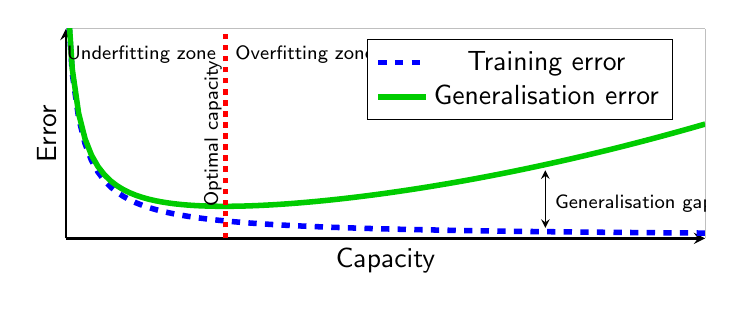
\begin{tikzpicture}[font=\sffamily\sansmath]

    \begin{axis}
        [
        xmin=0,
        xmax=2,
        ymin=0,
        ymax=2,
        xlabel=Capacity,
        ylabel=Error,
        ticks=none,
        xtick={2},
        ytick={2},
        xticklabels={\empty},
        yticklabels={\empty},
        ymajorgrids=true,
        xmajorgrids=true,
        width=0.8\linewidth,
        height=0.35\linewidth,
        axis line style = thick,
        legend style={at={(0.95,0.95)},anchor=north east}
        ]
        \addplot[domain=0.00:2.0, blue, dashed] {0.25/(3*x+0.1) + 0.01};   % Training error
        \addlegendentry{Training error}
        \addplot[domain=0.00:2.0, green!80!black] {0.25/(3*x+0.1) + 0.1*x + 0.2 *x*x + 0.05};  % Generalisation error
        \addlegendentry{Generalisation error}
%      \addplot[domain=0.39:1.61,black] {3*(x-2)*x+3.8};  %Total error
        \addplot[dotted, red] coordinates {(0.5,0) (0.5,2)};           %Optimum model complexity
        \addplot[thin, <->] coordinates {(1.5,0.1) (1.5,0.65)};       %Optimum model complexity

        \node[OptimumStyle] at (axis cs:0.46,1.0) {Optimal capacity};
        \node[UnderfitStyle] at (axis cs:0.5,1.75) {Underfitting zone};
        \node[OverfitStyle] at (axis cs:0.5,1.75) {Overfitting zone};
        \node[OverfitStyle] at (axis cs:1.5,0.33) {Generalisation gap};
%      \node[anchor=south west,text=Maroon] at (axis cs:1.4,0.4){Bias\textsuperscript{2}};
%      \node[anchor=north west,text=TealBlue] at (axis cs:1.4,0.85){Variance};
%      \node[anchor=south east,align=center] at (axis cs:1.5,1.5){Total\\error};
%        \legend{}
    \end{axis}
\end{tikzpicture}
%}

%\end{document}
    \captionsetup{format=hang} % hanging captions
    \caption{
        Typical relationship between capacity and error. Training and test error
        behave differently. At the left end of the graph, training error and
        generalization error are both high. This is the \textbf{underfitting
        regime} As we increase capacity, training error decreases, but the gap
        between training and generalisation error increases. Eventually, the
        size of this gap outweighs the decrease in training error, and we enter
        the \textbf{overfitting regime}, where capacity is too large, above the
        \textbf{optimal capacity}. Adapted from Goodfellow et. al.
        \cite{Goodfellow-et-al-2016}.
    }
    \label{fig:capacity}
\end{figure}

\subsubsection{No Free Lunch Theorem}
%%%%%%%%%%%%%%%%%%%%%%%%%%%%%%%%%%%%%%%%%%%%%%%%%%%%%%%%%%%%%%%%%%%%%%%%%%%%%%%%

The \gls{NFLT}, sometimes abbreviated NFL, is a simple but important concept in
\gls{ML} and optimisation. The theorem suggests that an optimisation technique
will perform equally well as any other when averaging its performance over the
set of all possible problems. This implies that there is no single best
technique for addressing an arbitrary problem. Luke states the following in
\textit{essentials of metaheuristics}~\cite{luke2012essentials}:

\begin{quotation}
    \textit{
        The NFL stated that within certain constraints, over the space of all
        possible problems, every optimization technique will perform as well as
        every other one on average (including Random Search)
    }
\end{quotation}

This argues that without having substantive information about the fundamentals
of the problem being modelled, choosing to apply a single technique to an
arbitrary problem will not yield a predictably better or worse result than
applying another to the same problem. Therefore, in the case where the
underlying process being optimised is not well-understood, a variety of
techniques should be applied.

However, in practice, knowledge to some degree is known about the problem which
is being optimised, or to which a learning algorithm is being applied. This
theorem highlights the importance of having a clear understanding of the problem
at hand before applying a learning algorithm or an optimisation technique. As
stated by Domingos~\cite{Domingos15}:

\begin{quotation}
    \textit{
        In the meantime, the practical consequence of the “no free lunch”
        theorem is that there’s no such thing as learning without knowledge.
        Data alone is not enough.
    }
\end{quotation}

This theorem, in effect, motivates the true goal of machine learning, as worded
by Goodfellow et. al.~\cite[p.~116]{Goodfellow-et-al-2016}:

\begin{quotation}
    \textit{
        This means that the goal of machine learning research is not to seek a
        universal learning algorithm or the absolute best learning algorithm.
        Instead, our goal is to understand what kinds of distributions are
        relevant to the “real world” that an AI agent experiences, and what
        kinds of machine learning algorithms perform well on data drawn from the
        kinds of data-generating distributions we care about.
    }
\end{quotation}

\subsubsection{Regularization}
%%%%%%%%%%%%%%%%%%%%%%%%%%%%%%%%%%%%%%%%%%%%%%%%%%%%%%%%%%%%%%%%%%%%%%%%%%%%%%%%

Regularization is any modification we make to a learning algorithm that is
intended to reduce its generalization error but not its training error

\subsection{Hyperparameters and Validation Sets}
%%%%%%%%%%%%%%%%%%%%%%%%%%%%%%%%%%%%%%%%%%%%%%%%%%%%%%%%%%%%%%%%%%%%%%%%%%%%%%%%

%\subsubsection{Resubstitution}
%%%%%%%%%%%%%%%%%%%%%%%%%%%%%%%%%%%%%%%%%%%%%%%%%%%%%%%%%%%%%%%%%%%%%%%%%%%%%%%%

%\subsubsection{Holdout}
%%%%%%%%%%%%%%%%%%%%%%%%%%%%%%%%%%%%%%%%%%%%%%%%%%%%%%%%%%%%%%%%%%%%%%%%%%%%%%%%

\subsubsection{Cross-Validation}
%%%%%%%%%%%%%%%%%%%%%%%%%%%%%%%%%%%%%%%%%%%%%%%%%%%%%%%%%%%%%%%%%%%%%%%%%%%%%%%%

\begin{figure}[htbp]
    \centering
    % DEP
% \usetikzlibrary{matrix}

% ACK
% https://tex.stackexchange.com/questions/429451/k-fold-cross-validation-figure-using-tikz-or-table

\begin{tikzpicture}
    \matrix (M)
        [
        matrix of nodes,
        nodes={
            minimum height = 6mm,
            minimum width = 1.3cm,
            outer sep=0,
            anchor=center,
            draw
        },
        column 1/.style={nodes={draw=none}, minimum width = 4cm},
        column 5/.style={nodes={draw=gray}, dashed},
        column 7/.style={nodes={draw=none},minimum width = 1.0cm},
        row 4/.style={nodes={draw=none}},
        row sep=1mm,
        column sep=-\pgflinewidth,
        nodes in empty cells,
        e/.style={fill=yellow!10},
        n/.style={nodes={draw=none, fill=none}},
        ]
    {
        Iteration 1   & |[e]|  &        &        & $\ldots$ &        & \textrightarrow\;$e_1$ \\
        Iteration 2   &        & |[e]|  &        & $\ldots$ &        & \textrightarrow\;$e_2$ \\
        Iteration 3   &        &        & |[e]|  & $\ldots$ &        & \textrightarrow\;$e_3$ \\
              $\vdots$  & $\vdots$ & $\vdots$ & $\vdots$ & $\ddots$ & $\vdots$ & $\vdots$                \\
        Iteration $k$ &        &        &        & $\ldots$ & |[e]|  & \textrightarrow\;$e_k$ \\
    };
    \draw (M-1-2.north west) ++(0,2mm) coordinate (LT) edge[|<->|, >= latex] node[above]{Total number of folds, $k$} (LT-|M-1-6.north east);
%    \draw[decorate,decoration = {brace}] (bias-brace-down) --  (bias-brace-up);
    \draw[decorate,decoration = {brace, raise=0.5em, amplitude=0.5em}]
        (M-5-6.south east)
        -- node[below=1em, align=center] {Validation \\ fold}
        ([shift={(0.1em,0)}]M-5-6.south west);

    \draw[decorate,decoration = {brace, raise=0.5em, amplitude=0.5em}]
        ([shift={(-0.1em,0)}]M-5-5.south east)
        -- node[below=1em, align=center] {Training folds}
        (M-5-2.south west);

    \draw[decorate,decoration = {brace, raise=0.5em, amplitude=0.5em}]
        (M.north east)
        -- node[midway, right=1.5em] {$e=\frac{1}{k}\sum_{i=0}^k{e_i}$}
        (M.south east);

%    \matrix (L)
%        [
%        matrix of nodes,
%        right=of M,
%        nodes={
%            minimum height = 6mm,
%            minimum width = 1.5cm,
%            outer sep=0,
%            anchor=center,
%            draw
%        },
%        column 1/.style={nodes={draw=none}, minimum width = 4cm},
%        row sep=1mm,
%        column sep=-\pgflinewidth,
%        nodes in empty cells,
%        e/.style={fill=yellow!10}
%        ]
%    {
%        Training   &       \\
%        Validation & |[e]| \\
%    };

%    \node[east=of M.east] {
%    \hskip1em
%    \begin{tabular}[c]{|p{2em}|l}
%      \cline{1-1}
%      \ccell{0}{1}  & Training
%      \nextrow{1-1}
%      \ccell{1}{1}  & Validation\\
%      \cline{1-1}
%    \end{tabular}
%    }
\end{tikzpicture}
    \captionsetup{format=hang} % hanging captions
    \caption{
        $k$-fold cross-validation procedure: (1) Dataset is divided into
        $k$-folds of roughly equal size. (2) Choose one fold randomly to be the
        holdout set then fit model on the remaining $k-1$ folds. (3) Iterate
        through the remaining $k-1$ folds, using each as the holdout set and
        record the error $e_i$ of the iteration. (4) Average the errors obtained
        over the $k$-folds.
    }
    \label{fig:kfold-cv}
\end{figure}

%\subsubsection{Leave-One-Out Cross-Validation (LOOCV)}
%%%%%%%%%%%%%%%%%%%%%%%%%%%%%%%%%%%%%%%%%%%%%%%%%%%%%%%%%%%%%%%%%%%%%%%%%%%%%%%%

%\subsubsection{Bootstrapping}
%%%%%%%%%%%%%%%%%%%%%%%%%%%%%%%%%%%%%%%%%%%%%%%%%%%%%%%%%%%%%%%%%%%%%%%%%%%%%%%%

%\subsection{Supervised}
%%%%%%%%%%%%%%%%%%%%%%%%%%%%%%%%%%%%%%%%%%%%%%%%%%%%%%%%%%%%%%%%%%%%%%%%%%%%%%%%


\section{Deep Learning\label{sec:DL}}
%%%%%%%%%%%%%%%%%%%%%%%%%%%%%%%%%%%%%%%%%%%%%%%%%%%%%%%%%%%%%%%%%%%%%%%%%%%%%%%%
\Gls{DL} is a field of \gls{ML} that is primarily concerned with
the learning of representations of data. The main idea is to use a \gls{NN} to learn representations of data. The main difference between a
\gls{NN} and a traditional \gls{ML} algorithm is that the
neural network is a function of the data, rather than the data itself.

\subsection{The fundamental component: Perceptrons}
%%%%%%%%%%%%%%%%%%%%%%%%%%%%%%%%%%%%%%%%%%%%%%%%%%%%%%%%%%%%%%%%%%%%%%%%%%%%%%%%

Proposed by Rosenblatt \cite{Rosenblatt_1957_6098} in his technical
report funded by the United States Office of Naval Research
\cite{doi:10.1177/030631296026003005} in 1957, the \textit{perceptron} is a
fundamental component of deep learning, describing a mathematical model of a
biological neuron. There are two different sets of notation which exist when
dealing with the bias of a perceptron. One involves the inclusion of a unit
constant in the input vector $\mathbf{x}$, with the bias being specified by the
value of the first weight $w_0$. An alternative notation exists which treats the
bias as a standalone value $b$. The latter notation will be used, as it is the
preferred notation in contemporary deep learning papers. The notation defining
the mapping of a perceptron is then: $f(\mathbf{x};\mathbf{w},
b)=\mathbf{x}^T\mathbf{w}+b$; $x\in\mathbb{R}^{d_{in}}$,
$\mathbf{w}\in\mathbb{R}^{d_{in}}$, $b\in\mathbb{R}$.

\begin{figure}[htbp]
    \centering
    % MIT License
%
% Copyright (c) 2021 Geoffrey H. Garrett
%
% Permission is hereby granted, free of charge, to any person obtaining a copy
% of this software and associated documentation files (the "Software"), to deal
% in the Software without restriction, including without limitation the rights
% to use, copy, modify, merge, publish, distribute, sublicense, and/or sell
% copies of the Software, and to permit persons to whom the Software is
% furnished to do so, subject to the following conditions:
%
% The above copyright notice and this permission notice shall be included in all
% copies or substantial portions of the Software.
%
% THE SOFTWARE IS PROVIDED "AS IS", WITHOUT WARRANTY OF ANY KIND, EXPRESS OR
% IMPLIED, INCLUDING BUT NOT LIMITED TO THE WARRANTIES OF MERCHANTABILITY,
% FITNESS FOR A PARTICULAR PURPOSE AND NONINFRINGEMENT. IN NO EVENT SHALL THE
% AUTHORS OR COPYRIGHT HOLDERS BE LIABLE FOR ANY CLAIM, DAMAGES OR OTHER
% LIABILITY, WHETHER IN AN ACTION OF CONTRACT, TORT OR OTHERWISE, ARISING FROM,
% OUT OF OR IN CONNECTION WITH THE SOFTWARE OR THE USE OR OTHER DEALINGS IN THE
% SOFTWARE.

%%%%%%%%%%%%%%%%%%%%%%%%%%%%%%%%%%%%%%%%%%%%%%%%%%%%%%%%%%%%%%%%%%%%%%%%%%%%%%%
% ACKNOWLEDGEMENTS
%%%%%%%%%%%%%%%%%%%%%%%%%%%%%%%%%%%%%%%%%%%%%%%%%%%%%%%%%%%%%%%%%%%%%%%%%%%%%%%
% Design and implementation of this diagram was inspired and adapted from:
% https://tex.stackexchange.com/questions/104334/tikz-diagram-of-a-perceptron

%%%%%%%%%%%%%%%%%%%%%%%%%%%%%%%%%%%%%%%%%%%%%%%%%%%%%%%%%%%%%%%%%%%%%%%%%%%%%%%
% DEPENDENCIES
%%%%%%%%%%%%%%%%%%%%%%%%%%%%%%%%%%%%%%%%%%%%%%%%%%%%%%%%%%%%%%%%%%%%%%%%%%%%%%%
%\usepackage{tikz}
%\usetikzlibrary{decorations.pathreplacing}    % for TikZ braces
%\usetikzlibrary{positioning}                  % for TikZ relative positioning

%%%%%%%%%%%%%%%%%%%%%%%%%%%%%%%%%%%%%%%%%%%%%%%%%%%%%%%%%%%%%%%%%%%%%%%%%%%%%%%
% USER STYLING
%%%%%%%%%%%%%%%%%%%%%%%%%%%%%%%%%%%%%%%%%%%%%%%%%%%%%%%%%%%%%%%%%%%%%%%%%%%%%%%

% TikZ node design.
\tikzset{basic/.style={draw,text width=1em,text badly centered}}
\tikzset{input/.style={}}
\tikzset{output/.style={}}
\tikzset{weight/.style={basic,circle}}
\tikzset{hidden/.style={basic,circle}}
\tikzset{function/.style={basic,circle}}

% Labels and symbols.
\def\activationlabel{activation function}  % activation function label
\def\activationsymbol{$\phi$}              % activation function symbol
\def\transferlabel{transfer function}      % transfer function label
\def\transfersymbol{$\sum$}                % transfer function symbol
\def\outputsymbol{$y$}                     % output symbol
\def\inputsymbol{$x$}                      % input symbol
\def\inputvecsymbol{$\mathbf{x}$}          % input vector symbol
\def\weightslabel{weights}                 % input vector symbol
\def\biassymbol{$b$}                       % bias symbol

%%%%%%%%%%%%%%%%%%%%%%%%%%%%%%%%%%%%%%%%%%%%%%%%%%%%%%%%%%%%%%%%%%%%%%%%%%%%%%%
% TIKZ PICTURE
%%%%%%%%%%%%%%%%%%%%%%%%%%%%%%%%%%%%%%%%%%%%%%%%%%%%%%%%%%%%%%%%%%%%%%%%%%%%%%%
\begin{tikzpicture}
    \usetikzlibrary{decorations.pathreplacing}    % for TikZ braces
    \usetikzlibrary{positioning}                  % for TikZ relative positioning

    \node[function] at (\transferx, -{int(2)})  (transfer) {\transfersymbol};
    \node[function, right=3em of transfer] (activation) {\activationsymbol};
    \node[below of=activation,font=\scriptsize,text width=3em] {\activationlabel};
    \node[below of=transfer,font=\scriptsize,text width=3em] {\transferlabel};
    \node[output, right=\layersep of activation] (output) {\outputsymbol};
    \path[draw,->] (transfer) -- (activation);
    \path[draw,->] (activation) -- (output);

    % Iterate through each row of units.
    \foreach \n [evaluate=\n as \p using {int(\n-1)}] in {0,1,2,3,4} {
        \ifnum \n=0
        \node[input] at (0, -\n) (X-\n) {$1$};
        \node[weight] at (\layersep, -\n) (W-\n) {$w_\n$};
        \else \ifnum \n=3
        \node[] at (0, -\n) (X-\n) {$\vdots$};
        \node[] at (\layersep, -\n) (W-\n) {$\vdots$};
        \else \ifnum \n=4
        \node[input] at (0, -\n) (X-\n) {$x_{d_{{in}}}$};
        \node[weight,label={[xshift=-0.0em]center:$w_{d_{{in}}}$}] at (\layersep, -\n) (W-\n) {\phantom{$w_{d_{{in}}}$}};
        \else
        \node[input] at (0, -\n) (X-\n) {$x_\n$};
        \node[weight] at (\layersep, -\n) (W-\n) {$w_\n$};
        \fi
        \fi
        \fi

        % Arrow from input to weight.
        \ifnum \n=3
        \else
        \path[draw,->] (X-\n) -- (W-\n);
                    \path[draw,->] (W-\n) -- (transfer);
        \fi

    }

    % Brace for bias.
    \node[left=1em of X-0] (bias-brace) {};
    \node[above=1em of bias-brace] (bias-brace-up) {};
    \node[below=1em of bias-brace] (bias-brace-down) {};
    \draw[decorate,decoration = {brace}] (bias-brace-down) --  (bias-brace-up);
    \node[left of=bias-brace,font=\scriptsize] {bias, \biassymbol};

    % Brace for input.
    \node[below=10em of bias-brace-down] (input-brace-down) {};
    \node[below=5em of bias-brace-down] (input-brace) {};
    \draw[decorate,decoration = {brace}] (input-brace-down) --  (bias-brace-down);
    \node[left of=input-brace,font=\scriptsize] {inputs, \inputvecsymbol};

    % Weights label.
    \node[below of=W-4,font=\scriptsize] {\weightslabel};

\end{tikzpicture}

    \caption{Perceptron}
    \label{fig:perceptron}
\end{figure}

This mathematical mimicry of a biological neuron was first used used proposed by
Rosenblatt where a set of inputs $\mathbf{x}$ weighted using $\mathbf{w}$ before
being summed. If this sum surpassed a threshold, then a binary output of $1$ was
returned. \autoref{fig:perceptron} shows a more general formulation which
applies to the resulting field of deep learning, with any activation function
$\phi$ analogous for the level of excitation of a biological neuron in response
to its stimulus $\mathbf{x}$.

The primary criticism of the perceptron came in 1969 from Minsky and Papert
\cite{minsky69perceptrons}, where it was shown that the perceptron could only
solve \textit{linearly separable} functions, and failed to solve the XOR and
NXOR functions. They went on to claim that the research being done was doomed to
failure due to these limitations, resulting in little research in the area being
done until about the 1980's.

\subsection{Activation function}
%%%%%%%%%%%%%%%%%%%%%%%%%%%%%%%%%%%%%%%%%%%%%%%%%%%%%%%%%%%%%%%%%%%%%%%%%%%%%%%%

Since the early days of the perceptron, a wide variety of activation functions
$\phi$ have been used and improve upon the threshold step function.

%\begin{figure}[htbp]
%    \centering
%    \makeatletter
\pgfmathdeclarefunction{erf}{1}{%
    \begingroup
    \pgfmathparse{#1 > 0 ? 1 : -1}%
    \edef\sign{\pgfmathresult}%
    \pgfmathparse{abs(#1)}%
    \edef\x{\pgfmathresult}%
    \pgfmathparse{1/(1+0.3275911*\x)}%
    \edef\t{\pgfmathresult}%
    \pgfmathparse{%
        1 - (((((1.061405429*\t -1.453152027)*\t) + 1.421413741)*\t
        -0.284496736)*\t + 0.254829592)*\t*exp(-(\x*\x))}%
    \edef\y{\pgfmathresult}%
    \pgfmathparse{(\sign)*\y}%
    \pgfmath@smuggleone\pgfmathresult%
    \endgroup
}
%dep
%subfig
\begin{figure}[htp]
    \centering
    \captionsetup{format=hang} % hanging captions
    \subfloat[Threshold Step]{
        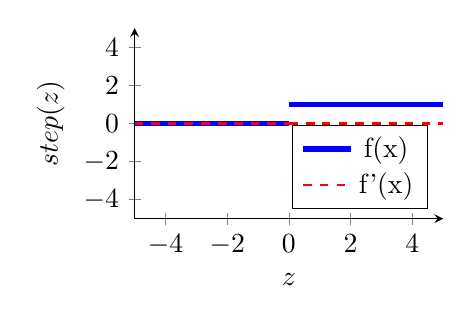
\begin{tikzpicture}
            \label{fig:threshold}
            \begin{axis}
                [width=5.5cm,height=4cm,ylabel=$step(z)$,xlabel=$z$,ymin=-5.0,ymax=5.0,xmin=-5,xmax=5,
                legend style={at={(0.95,0.05)},anchor=south east},]
                \addplot[blue,smooth, domain=-5:0] {0};
                \addplot[red,dashed, thick, domain=-5:0] {0};
                \addplot[blue,smooth, domain=-0:5] {1};
                \addplot[red,dashed, thick, domain=-0:5] {0};
                \addlegendentry{f(x)}
                \addlegendentry{f'(x)}
            \end{axis}
        \end{tikzpicture}
    }
    \subfloat[Linear]{
        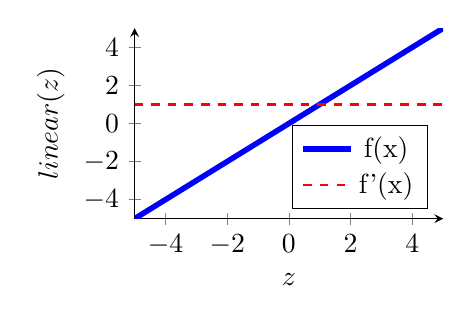
\begin{tikzpicture}
            \label{fig:linear}
            \begin{axis}
                [width=5.5cm,height=4cm,ylabel=$linear(z)$,xlabel=$z$,ymin=-5.0,ymax=5.0,xmin=-5,xmax=5,
                legend style={at={(0.95,0.05)},anchor=south east},]
                \addplot[blue,smooth] {x};
                \addlegendentry{f(x)}
                \addplot[red,dashed, thick] {1};
                \addlegendentry{f'(x)}
            \end{axis}
        \end{tikzpicture}
    }
    \subfloat[Sigmoid]{
        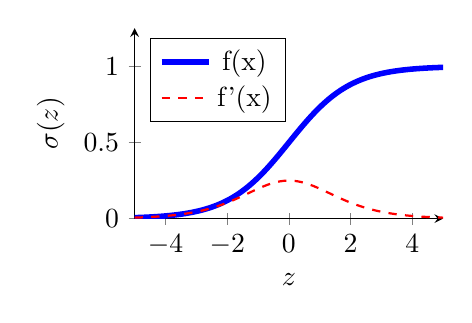
\begin{tikzpicture}
            \label{fig:sigmoid}
            \begin{axis}
                [width=5.5cm,height=4cm,ylabel=$\sigma(z)$,xlabel=$z$,ymin=0,ymax=1.25,xmin=-5,xmax=5,
                legend style={at={(0.05,0.95)},anchor=north west},]
                \addplot[blue,smooth] {1/(1+exp(-x))};
                \addlegendentry{f(x)}
                \addplot[red, dashed, thick] {1/(1+exp(-x)) * (1-1/(1+exp(-x)))};
                \addlegendentry{f'(x)}
            \end{axis}
        \end{tikzpicture}
    }\\
    \subfloat[Hyperbolic tangent]{
        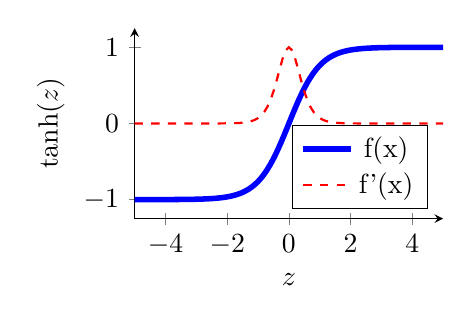
\begin{tikzpicture}
            \label{fig:hyperbolic_tangent}
            \begin{axis}
                [width=5.5cm,height=4cm,ylabel=$\tanh(z)$,xlabel=$z$,ymin=-1.25,ymax=1.25,xmin=-5,xmax=5, legend style={at={(0.95,0.05)},anchor=south east},]
                \addplot[blue,smooth] {tanh(x)};
                \addlegendentry{f(x)}
                \addplot[red,dashed, thick] {1/cosh(2*x)*1/cosh(2*x)};
                \addlegendentry{f'(x)}
            \end{axis}
        \end{tikzpicture}
    }
    \subfloat[ReLU]{
        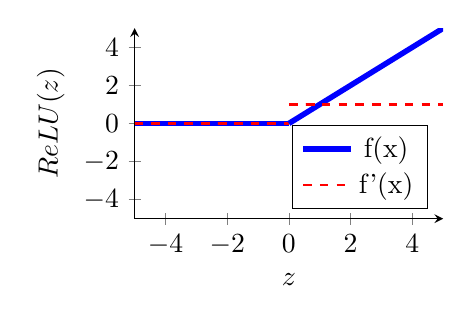
\begin{tikzpicture}
            \label{fig:relu}
            \begin{axis}
                [width=5.5cm,height=4cm,ylabel=$ReLU(z)$,xlabel=$z$,ymin=-5.0,ymax=5.0,xmin=-5,xmax=5,
                legend style={at={(0.95,0.05)},anchor=south east},]
                \addplot[blue,smooth, domain=-5:0] {0};
                \addplot[red,dashed, thick, domain=-5:0] {0};
                \addplot[blue,smooth, domain=-0:5] {x};
                \addplot[red,dashed, thick, domain=-0:5] {1};
                \addlegendentry{f(x)}
                \addlegendentry{f'(x)}
            \end{axis}
        \end{tikzpicture}
    }
    \subfloat[Leaky ReLU]{
        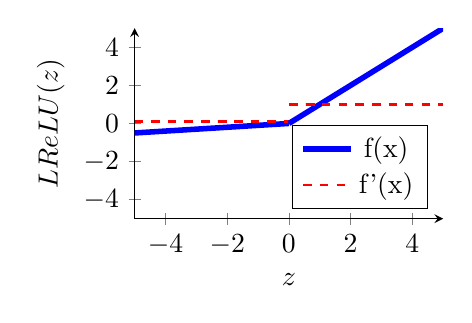
\begin{tikzpicture}
            \label{fig:lrelu}
            \begin{axis}
                [width=5.5cm,height=4cm,ylabel=$LReLU(z)$,xlabel=$z$,ymin=-5.0,ymax=5.0,xmin=-5,xmax=5,
                legend style={at={(0.95,0.05)},anchor=south east},]
                \addplot[blue,smooth, domain=-5:0] {0.1*x};
                \addplot[red,dashed, thick, domain=-5:0] {0.1};
                \addplot[blue,smooth, domain=-0:5] {x};
                \addplot[red,dashed, thick, domain=-0:5] {1};
                \addlegendentry{f(x)}
                \addlegendentry{f'(x)}
            \end{axis}
        \end{tikzpicture}
    }\\
    \subfloat[GELU]{
        \begin{tikzpicture}
            \label{fig:gelu}
            \begin{axis}
                [width=5.5cm,height=4cm,ylabel=$GELU(z)$,xlabel=$z$,ymin=-5.0,ymax=5.0,xmin=-5,xmax=5,
                legend style={at={(0.95,0.05)},anchor=south east},]
                \addplot[blue,smooth] {x * 0.5 * (1 + erf(x /sqrt(2)))};
                \addplot[red,dashed, thick] {0.5 * (1 + erf(x /sqrt(2))) + 1/sqrt(2*pi) * (exp(-x*x/2))};
                \addlegendentry{f(x)}
                \addlegendentry{f'(x)}
            \end{axis}
        \end{tikzpicture}
    }
    \subfloat[Swish]{
        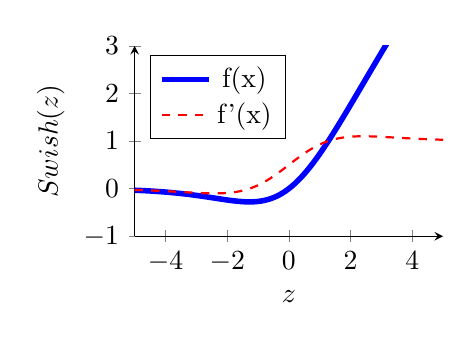
\begin{tikzpicture}
            \label{fig:swish}
            \begin{axis}
                [width=5.5cm,height=4cm,ylabel=$Swish(z)$,xlabel=$z$,ymin=-1,ymax=3.0,xmin=-5,xmax=5,
                legend style={at={(0.05,0.95)},anchor=north west},]
                \addplot[blue,smooth] {x*(1/(1+exp(-x)))}; % f (x) + σ (x) (1 − f (x))
                \addlegendentry{f(x)}
                \addplot[red, dashed, thick] {x/(1+exp(-x)) + 1/(1+exp(-x)) * (1-x/(1+exp(-x)))};
                \addlegendentry{f'(x)}
            \end{axis}
        \end{tikzpicture}
    }
    \subfloat[SIREN]{
        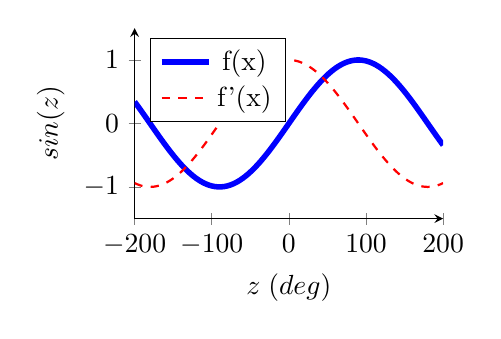
\begin{tikzpicture}
            \label{fig:siren}
            \begin{axis}
                [width=5.5cm,height=4cm,ylabel=$sin(z)$,xlabel=$z\;\text{(deg)}$,ymin=-1.5,ymax=1.5,xmin=-200,xmax=200,
                legend style={at={(0.05,0.95)},anchor=north west},]
                \addplot[blue,smooth,domain=-200:200] {sin(x)}; % f (x) + σ (x) (1 − f (x))
                \addlegendentry{f(x)}
                \addplot[red, dashed, thick,domain=-200:200] {cos(x)};
                \addlegendentry{f'(x)}
            \end{axis}
        \end{tikzpicture}
    }
    \caption[Activation functions.]{\textbf{Activation functions} used in \gls{DL}, included for results in their performance or historic significance in the applications of artificial neural networks.}
    \label{fig:activation-functions}
\end{figure}
%    \caption{Activation functions}
%    \label{fig:activation}
%\end{figure}
\makeatletter
\pgfmathdeclarefunction{erf}{1}{%
    \begingroup
    \pgfmathparse{#1 > 0 ? 1 : -1}%
    \edef\sign{\pgfmathresult}%
    \pgfmathparse{abs(#1)}%
    \edef\x{\pgfmathresult}%
    \pgfmathparse{1/(1+0.3275911*\x)}%
    \edef\t{\pgfmathresult}%
    \pgfmathparse{%
        1 - (((((1.061405429*\t -1.453152027)*\t) + 1.421413741)*\t
        -0.284496736)*\t + 0.254829592)*\t*exp(-(\x*\x))}%
    \edef\y{\pgfmathresult}%
    \pgfmathparse{(\sign)*\y}%
    \pgfmath@smuggleone\pgfmathresult%
    \endgroup
}
%dep
%subfig
\begin{figure}[htp]
    \centering
    \captionsetup{format=hang} % hanging captions
    \subfloat[Threshold Step]{
        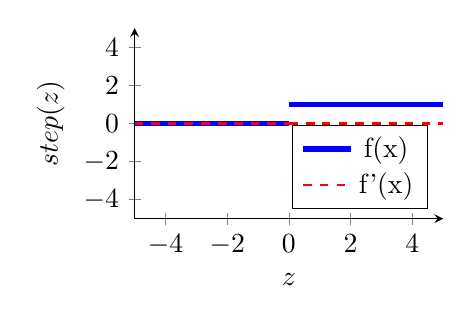
\begin{tikzpicture}
            \label{fig:threshold}
            \begin{axis}
                [width=5.5cm,height=4cm,ylabel=$step(z)$,xlabel=$z$,ymin=-5.0,ymax=5.0,xmin=-5,xmax=5,
                legend style={at={(0.95,0.05)},anchor=south east},]
                \addplot[blue,smooth, domain=-5:0] {0};
                \addplot[red,dashed, thick, domain=-5:0] {0};
                \addplot[blue,smooth, domain=-0:5] {1};
                \addplot[red,dashed, thick, domain=-0:5] {0};
                \addlegendentry{f(x)}
                \addlegendentry{f'(x)}
            \end{axis}
        \end{tikzpicture}
    }
    \subfloat[Linear]{
        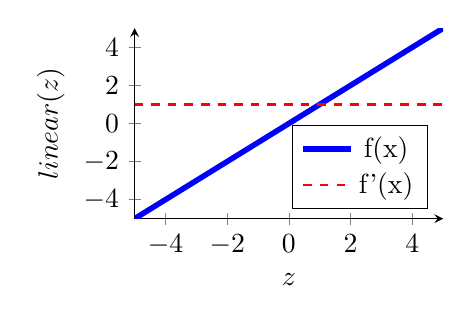
\begin{tikzpicture}
            \label{fig:linear}
            \begin{axis}
                [width=5.5cm,height=4cm,ylabel=$linear(z)$,xlabel=$z$,ymin=-5.0,ymax=5.0,xmin=-5,xmax=5,
                legend style={at={(0.95,0.05)},anchor=south east},]
                \addplot[blue,smooth] {x};
                \addlegendentry{f(x)}
                \addplot[red,dashed, thick] {1};
                \addlegendentry{f'(x)}
            \end{axis}
        \end{tikzpicture}
    }
    \subfloat[Sigmoid]{
        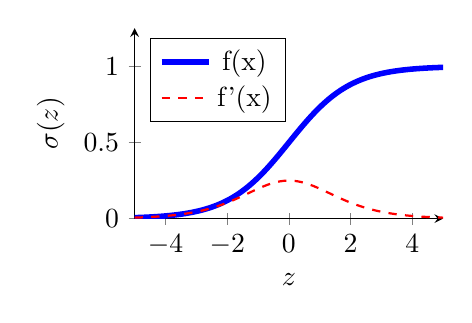
\begin{tikzpicture}
            \label{fig:sigmoid}
            \begin{axis}
                [width=5.5cm,height=4cm,ylabel=$\sigma(z)$,xlabel=$z$,ymin=0,ymax=1.25,xmin=-5,xmax=5,
                legend style={at={(0.05,0.95)},anchor=north west},]
                \addplot[blue,smooth] {1/(1+exp(-x))};
                \addlegendentry{f(x)}
                \addplot[red, dashed, thick] {1/(1+exp(-x)) * (1-1/(1+exp(-x)))};
                \addlegendentry{f'(x)}
            \end{axis}
        \end{tikzpicture}
    }\\
    \subfloat[Hyperbolic tangent]{
        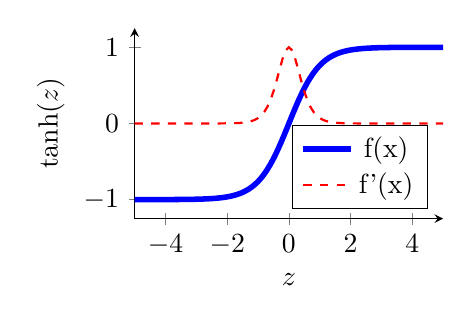
\begin{tikzpicture}
            \label{fig:hyperbolic_tangent}
            \begin{axis}
                [width=5.5cm,height=4cm,ylabel=$\tanh(z)$,xlabel=$z$,ymin=-1.25,ymax=1.25,xmin=-5,xmax=5, legend style={at={(0.95,0.05)},anchor=south east},]
                \addplot[blue,smooth] {tanh(x)};
                \addlegendentry{f(x)}
                \addplot[red,dashed, thick] {1/cosh(2*x)*1/cosh(2*x)};
                \addlegendentry{f'(x)}
            \end{axis}
        \end{tikzpicture}
    }
    \subfloat[ReLU]{
        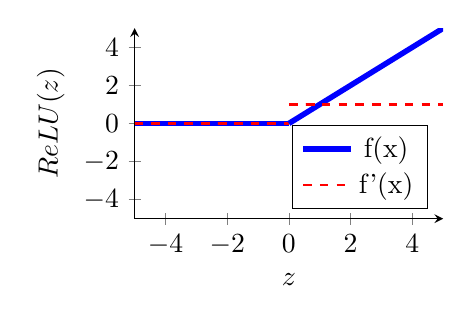
\begin{tikzpicture}
            \label{fig:relu}
            \begin{axis}
                [width=5.5cm,height=4cm,ylabel=$ReLU(z)$,xlabel=$z$,ymin=-5.0,ymax=5.0,xmin=-5,xmax=5,
                legend style={at={(0.95,0.05)},anchor=south east},]
                \addplot[blue,smooth, domain=-5:0] {0};
                \addplot[red,dashed, thick, domain=-5:0] {0};
                \addplot[blue,smooth, domain=-0:5] {x};
                \addplot[red,dashed, thick, domain=-0:5] {1};
                \addlegendentry{f(x)}
                \addlegendentry{f'(x)}
            \end{axis}
        \end{tikzpicture}
    }
    \subfloat[Leaky ReLU]{
        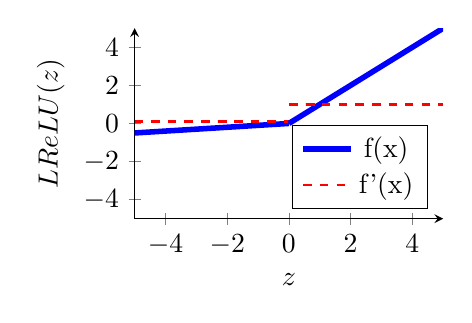
\begin{tikzpicture}
            \label{fig:lrelu}
            \begin{axis}
                [width=5.5cm,height=4cm,ylabel=$LReLU(z)$,xlabel=$z$,ymin=-5.0,ymax=5.0,xmin=-5,xmax=5,
                legend style={at={(0.95,0.05)},anchor=south east},]
                \addplot[blue,smooth, domain=-5:0] {0.1*x};
                \addplot[red,dashed, thick, domain=-5:0] {0.1};
                \addplot[blue,smooth, domain=-0:5] {x};
                \addplot[red,dashed, thick, domain=-0:5] {1};
                \addlegendentry{f(x)}
                \addlegendentry{f'(x)}
            \end{axis}
        \end{tikzpicture}
    }\\
    \subfloat[GELU]{
        \begin{tikzpicture}
            \label{fig:gelu}
            \begin{axis}
                [width=5.5cm,height=4cm,ylabel=$GELU(z)$,xlabel=$z$,ymin=-5.0,ymax=5.0,xmin=-5,xmax=5,
                legend style={at={(0.95,0.05)},anchor=south east},]
                \addplot[blue,smooth] {x * 0.5 * (1 + erf(x /sqrt(2)))};
                \addplot[red,dashed, thick] {0.5 * (1 + erf(x /sqrt(2))) + 1/sqrt(2*pi) * (exp(-x*x/2))};
                \addlegendentry{f(x)}
                \addlegendentry{f'(x)}
            \end{axis}
        \end{tikzpicture}
    }
    \subfloat[Swish]{
        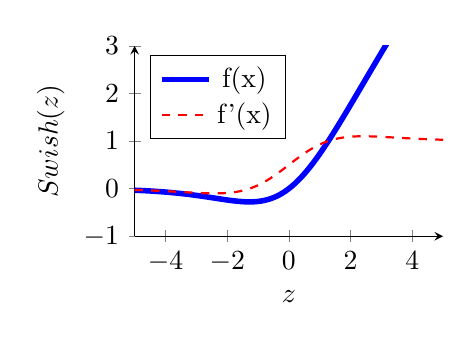
\begin{tikzpicture}
            \label{fig:swish}
            \begin{axis}
                [width=5.5cm,height=4cm,ylabel=$Swish(z)$,xlabel=$z$,ymin=-1,ymax=3.0,xmin=-5,xmax=5,
                legend style={at={(0.05,0.95)},anchor=north west},]
                \addplot[blue,smooth] {x*(1/(1+exp(-x)))}; % f (x) + σ (x) (1 − f (x))
                \addlegendentry{f(x)}
                \addplot[red, dashed, thick] {x/(1+exp(-x)) + 1/(1+exp(-x)) * (1-x/(1+exp(-x)))};
                \addlegendentry{f'(x)}
            \end{axis}
        \end{tikzpicture}
    }
    \subfloat[SIREN]{
        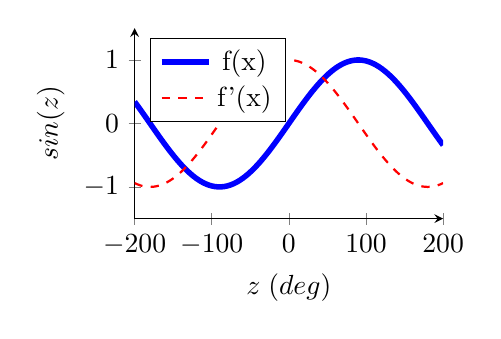
\begin{tikzpicture}
            \label{fig:siren}
            \begin{axis}
                [width=5.5cm,height=4cm,ylabel=$sin(z)$,xlabel=$z\;\text{(deg)}$,ymin=-1.5,ymax=1.5,xmin=-200,xmax=200,
                legend style={at={(0.05,0.95)},anchor=north west},]
                \addplot[blue,smooth,domain=-200:200] {sin(x)}; % f (x) + σ (x) (1 − f (x))
                \addlegendentry{f(x)}
                \addplot[red, dashed, thick,domain=-200:200] {cos(x)};
                \addlegendentry{f'(x)}
            \end{axis}
        \end{tikzpicture}
    }
    \caption[Activation functions.]{\textbf{Activation functions} used in \gls{DL}, included for results in their performance or historic significance in the applications of artificial neural networks.}
    \label{fig:activation-functions}
\end{figure}

\subsection{Multilayer perceptrons, a.k.a feed forward networks}
%%%%%%%%%%%%%%%%%%%%%%%%%%%%%%%%%%%%%%%%%%%%%%%%%%%%%%%%%%%%%%%%%%%%%%%%%%%%%%%%

$f(\mathbf{x};\mathbf{w}, b)=\mathbf{x}^T\mathbf{w}+b$; $x\in\mathbb{R}^{d_{in}}$, $\mathbf{w}\in\mathbb{R}^{d_{in}\times}$, $b\in\mathbb{R}^1$.

\begin{figure}
    \centering
    % MIT License
%
% Copyright (c) 2021 Geoffrey H. Garrett
%
% Permission is hereby granted, free of charge, to any person obtaining a copy
% of this software and associated documentation files (the "Software"), to deal
% in the Software without restriction, including without limitation the rights
% to use, copy, modify, merge, publish, distribute, sublicense, and/or sell
% copies of the Software, and to permit persons to whom the Software is
% furnished to do so, subject to the following conditions:
%
% The above copyright notice and this permission notice shall be included in all
% copies or substantial portions of the Software.
%
% THE SOFTWARE IS PROVIDED "AS IS", WITHOUT WARRANTY OF ANY KIND, EXPRESS OR
% IMPLIED, INCLUDING BUT NOT LIMITED TO THE WARRANTIES OF MERCHANTABILITY,
% FITNESS FOR A PARTICULAR PURPOSE AND NONINFRINGEMENT. IN NO EVENT SHALL THE
% AUTHORS OR COPYRIGHT HOLDERS BE LIABLE FOR ANY CLAIM, DAMAGES OR OTHER
% LIABILITY, WHETHER IN AN ACTION OF CONTRACT, TORT OR OTHERWISE, ARISING FROM,
% OUT OF OR IN CONNECTION WITH THE SOFTWARE OR THE USE OR OTHER DEALINGS IN THE
% SOFTWARE.

%%%%%%%%%%%%%%%%%%%%%%%%%%%%%%%%%%%%%%%%%%%%%%%%%%%%%%%%%%%%%%%%%%%%%%%%%%%%%%%
% ACKNOWLEDGEMENTS
%%%%%%%%%%%%%%%%%%%%%%%%%%%%%%%%%%%%%%%%%%%%%%%%%%%%%%%%%%%%%%%%%%%%%%%%%%%%%%%
% Adapted from:
% https://www.researchgate.net/figure/The-agent-environment-interaction-in-reinforcement-learning_fig1_328494763

%%%%%%%%%%%%%%%%%%%%%%%%%%%%%%%%%%%%%%%%%%%%%%%%%%%%%%%%%%%%%%%%%%%%%%%%%%%%%%%
% DEPENDENCIES
%%%%%%%%%%%%%%%%%%%%%%%%%%%%%%%%%%%%%%%%%%%%%%%%%%%%%%%%%%%%%%%%%%%%%%%%%%%%%%%
%\usepackage{tikz}
%\usetikzlibrary{decorations.pathreplacing}    % for TikZ braces
%\usetikzlibrary{positioning}                  % for TikZ relative positioning

%%%%%%%%%%%%%%%%%%%%%%%%%%%%%%%%%%%%%%%%%%%%%%%%%%%%%%%%%%%%%%%%%%%%%%%%%%%%%%%
% USER STYLING
%%%%%%%%%%%%%%%%%%%%%%%%%%%%%%%%%%%%%%%%%%%%%%%%%%%%%%%%%%%%%%%%%%%%%%%%%%%%%%%

% TikZ node design.
\tikzset{basic/.style={draw,text width=1em,text badly centered}}
\tikzset{input/.style={basic, fill=green!25, circle}}
\tikzset{output/.style={basic, fill=blue!25, circle}}
\tikzset{weight/.style={basic,circle}}
\tikzset{hidden/.style={basic,circle}}
\tikzset{function/.style={basic,circle}}
\def\layersep{3em}
\def\transferx{9em}
\def\hiddenx{7em}
\def\hiddenxn{12em}


\def\sep{4em}
\def\L{\gls{L}}       % number of hidden layers
\def\y{\gls{y_true}}  % output vector
\def\x{\gls{ml:x}}    % input vector
\def\h{\gls{a_vec}}   % hidden output
\def\nx{\gls{ml:n_x}}   % hidden output
\def\ny{\gls{ml:n_y}}   % hidden output


%%%%%%%%%%%%%%%%%%%%%%%%%%%%%%%%%%%%%%%%%%%%%%%%%%%%%%%%%%%%%%%%%%%%%%%%%%%%%%%
% TIKZ PICTURE
%%%%%%%%%%%%%%%%%%%%%%%%%%%%%%%%%%%%%%%%%%%%%%%%%%%%%%%%%%%%%%%%%%%%%%%%%%%%%%%
\begin{tikzpicture}
    \usetikzlibrary{decorations.pathreplacing}    % for TikZ braces
    \usetikzlibrary{positioning}                  % for TikZ relative positioning

    % input
    \foreach \n/\p in {0/1,1/2,2/3,3/4,4/5} {
        \ifnum \n=3
            % dots layer
            \node[] at (0, -\n) (X_\n) {$\vdots$};
            \node[] at (\hiddenx, -\n) (H1_\n) {$\vdots$};
            \node[right of=H1_\n] (M-\n) {$\ddots$};
            \node[below of=H1_2] (H2_\n) {$\vdots$};
            \node[below of=H2_2] (H2_\n) {$\vdots$};
            \node[right=5.7em of H2_\n] (Y_\n) {$\vdots$};
        \else
        \ifnum \n=4
            % n layer
            \node[input] at (0, -\n) (X_\n) {};
            \node[left of=X_\n] (I_\n) {$x_{\nx}$};
            \path[draw,->] (I_\n) -- (X_\n);
            \node[hidden] at (\hiddenx, -\n) (H1_\n) {}; %{$h_{n, 1}$};
            \node[right of= H1_\n] (M-\n) {$\ldots$};
            \node[hidden, right of= M-\n] (H2_\n) {}; % {$h_{n, m}$};
            \node[output, right= 5em of H2_\n] (Y_\n) {}; % {$h_{n, m}$};
            \node[right of=Y_\n] (O_\n) {$y_{\ny}$};
            \path[draw,->] (Y_\n) -- (O_\n);
        \else
            \node[input] at (0, -{\n}) (X_\n) {};
            \node[left of=X_\n] (I_\n) {$x_{\p}$};
            \path[draw,->] (I_\n) -- (X_\n);
            \node[hidden] at (\hiddenx, -\n) (H1_\n) {};%{$h_{\n, 1}$};
            \node[right of=H1_\n] (M-\n) {$\ldots$};
            \node[hidden, right of=M-\n] (H2_\n) {};% {$h_{\n, m}$};
            \node[output, right= 5em of H2_\n] (Y_\n) {}; % {$h_{n, m}$};
            \node[right of=Y_\n] (O_\n) {$y_\p$};
            \path[draw,->] (Y_\n) -- (O_\n);
        \fi
        \fi
    }

    % input layer connected to first hidden layer
    \foreach \j in {0,1,2,4} {
        \foreach \n in {0,1,2,4} {
            \path[draw,->] (X_\n) -- (H1_\j);
        }
    }

    % second hidden layer connected to output layer
    \foreach \j in {0,1,2,4} {
        \foreach \n in {0,1,2,4} {
            \path[draw,->] (H2_\n) -- (Y_\j);
        }
    }

    % labels
    \node[below of=X_4,font=\scriptsize, align=center] {input\\layer};
    \node[below of=Y_4,font=\scriptsize, align=center] {output\\layer};

    % brace for hidden layers
    \node[below=1em of M-4] (hidden-brace) {};
    \node[right=3em of hidden-brace] (hidden-brace-right) {};
    \node[left=3em of hidden-brace] (hidden-brace-left) {};
    \draw [decorate,decoration = {brace}] (hidden-brace-right) --  (hidden-brace-left);
    \node[below=0.5em of hidden-brace,font=\scriptsize] (hlayer) {hidden layer(s)};

\end{tikzpicture}


    \caption{Multilayer perceptron}
    \label{fig:mlp}
\end{figure}


\begin{figure}
    \centering
    % MIT License
%
% Copyright (c) 2021 Geoffrey H. Garrett
%
% Permission is hereby granted, free of charge, to any person obtaining a copy
% of this software and associated documentation files (the "Software"), to deal
% in the Software without restriction, including without limitation the rights
% to use, copy, modify, merge, publish, distribute, sublicense, and/or sell
% copies of the Software, and to permit persons to whom the Software is
% furnished to do so, subject to the following conditions:
%
% The above copyright notice and this permission notice shall be included in all
% copies or substantial portions of the Software.
%
% THE SOFTWARE IS PROVIDED "AS IS", WITHOUT WARRANTY OF ANY KIND, EXPRESS OR
% IMPLIED, INCLUDING BUT NOT LIMITED TO THE WARRANTIES OF MERCHANTABILITY,
% FITNESS FOR A PARTICULAR PURPOSE AND NONINFRINGEMENT. IN NO EVENT SHALL THE
% AUTHORS OR COPYRIGHT HOLDERS BE LIABLE FOR ANY CLAIM, DAMAGES OR OTHER
% LIABILITY, WHETHER IN AN ACTION OF CONTRACT, TORT OR OTHERWISE, ARISING FROM,
% OUT OF OR IN CONNECTION WITH THE SOFTWARE OR THE USE OR OTHER DEALINGS IN THE
% SOFTWARE.

%%%%%%%%%%%%%%%%%%%%%%%%%%%%%%%%%%%%%%%%%%%%%%%%%%%%%%%%%%%%%%%%%%%%%%%%%%%%%%%
% DEPENDENCIES
%%%%%%%%%%%%%%%%%%%%%%%%%%%%%%%%%%%%%%%%%%%%%%%%%%%%%%%%%%%%%%%%%%%%%%%%%%%%%%%
%\usepackage{tikz}
%\usetikzlibrary{decorations.pathreplacing}    % for TikZ braces
%\usetikzlibrary{positioning}                  % for TikZ relative positioning

%%%%%%%%%%%%%%%%%%%%%%%%%%%%%%%%%%%%%%%%%%%%%%%%%%%%%%%%%%%%%%%%%%%%%%%%%%%%%%%
% USER STYLING
%%%%%%%%%%%%%%%%%%%%%%%%%%%%%%%%%%%%%%%%%%%%%%%%%%%%%%%%%%%%%%%%%%%%%%%%%%%%%%%

% TikZ node design.
\tikzset{basic/.style={draw,text badly centered}}
\tikzset{input/.style={basic,minimum width=1.2cm, fill=green!25, circle}}
\tikzset{output/.style={basic,minimum width=1.2cm, fill=blue!25, circle}}
\tikzset{weight/.style={basic,circle}}
\tikzset{hidden/.style={basic,circle, minimum width=1.2cm}}
\tikzset{function/.style={basic,circle}}

\def\sep{4em}
\def\L{\gls{L}}       % number of hidden layers
\def\y{\gls{y_pred}}  % output vector
\def\x{\gls{ml:x}}    % input vector
\def\h{\gls{a_vec}}   % hidden output

%%%%%%%%%%%%%%%%%%%%%%%%%%%%%%%%%%%%%%%%%%%%%%%%%%%%%%%%%%%%%%%%%%%%%%%%%%%%%%%
% TIKZ PICTURE
%%%%%%%%%%%%%%%%%%%%%%%%%%%%%%%%%%%%%%%%%%%%%%%%%%%%%%%%%%%%%%%%%%%%%%%%%%%%%%%
\begin{tikzpicture}
    \node[input, label={[xshift=-0.0em]center:\gls{dl:a:vec:0}}] (X) {\phantom{\gls{dl:a:vec:1}}};
    \node[, left=1.5em of X] (in) {$\bm{x}$};

    \node[hidden, right=\sep of X, label={[xshift=-0.0em]center:\gls{dl:a:vec:1}}] (H1) {\phantom{\gls{dl:a:vec:1}}};
    \node[hidden, right=\sep of H1, label={[xshift=-0.0em]center:\gls{dl:a:vec:Lm1}}] (H2) {\phantom{\gls{dl:a:vec:Lm1}}};
    \node[output, right=\sep of H2,  label={[xshift=-0.0em]center:\gls{dl:a:vec:L}}] (Y) {\phantom{\gls{dl:a:vec:L}}};
    \node[, right=1.5em of Y] (out) {$\bm{\hat{y}}$};

    \path[draw,->] (in) -- (X);
    \path[draw,->] (X) -- (H1);
    \node[right=0.8em of H1] (M) {$\ldots$};
    \path[draw,->] (H2) -- (Y);
    \path[draw,->] (Y) -- (out);
\end{tikzpicture}


    \caption{Multilayer perceptron}
    \label{fig:mlp-vec}
\end{figure}


\begin{equation}
    \mathbf{h}^{(1)} = g^{(1)} \bigg(\mathbf{W}^{{(1)}\;T}\mathbf{x} + \mathbf{b}^{(1)}\bigg);
\end{equation}

\begin{equation}
    \mathbf{h}^{(2)} = g^{(2)} \bigg(\mathbf{W}^{{(2)}\;T}\mathbf{h}^{(1)} + \mathbf{b}^{(2)}\bigg);
\end{equation}

\subsection{Gradient based learning}
%%%%%%%%%%%%%%%%%%%%%%%%%%%%%%%%%%%%%%%%%%%%%%%%%%%%%%%%%%%%%%%%%%%%%%%%%%%%%%%%

Backpropagation, short for "backward propagation of errors," is a
\textit{supervised learning} algorithm for artificial neural networks using
\textit{gradient descent}.

\begin{figure}[htp]
    \centering
    
% https://github.com/davidstutz/latex-resources/blob/master/tikz-gradient-descent/gradient-descent.tex
% \usepackage{tikz}
% \usepackage{tikz}
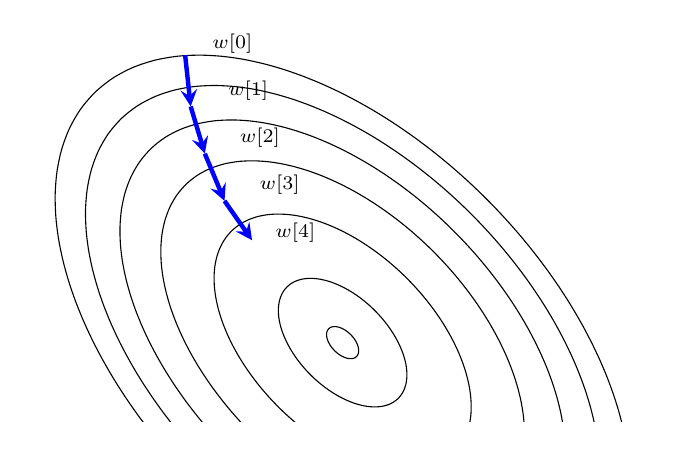
\begin{tikzpicture}[samples=100,smooth]
    \begin{scope}
        \clip(-4,-1) rectangle (4,4);
        \draw plot[domain=0:360] ({cos(\x)*sqrt(20/(sin(2*\x)+2))},{sin(\x)*sqrt(20/(sin(2*\x)+2))});
        \draw plot[domain=0:360] ({cos(\x)*sqrt(16/(sin(2*\x)+2))},{sin(\x)*sqrt(16/(sin(2*\x)+2))});
        \draw plot[domain=0:360] ({cos(\x)*sqrt(12/(sin(2*\x)+2))},{sin(\x)*sqrt(12/(sin(2*\x)+2))});
        \draw plot[domain=0:360] ({cos(\x)*sqrt(8/(sin(2*\x)+2))},{sin(\x)*sqrt(8/(sin(2*\x)+2))});
        \draw plot[domain=0:360] ({cos(\x)*sqrt(4/(sin(2*\x)+2))},{sin(\x)*sqrt(4/(sin(2*\x)+2))});
        \draw plot[domain=0:360] ({cos(\x)*sqrt(1/(sin(2*\x)+2))},{sin(\x)*sqrt(1/(sin(2*\x)+2))});
        \draw plot[domain=0:360] ({cos(\x)*sqrt(0.0625/(sin(2*\x)+2))},{sin(\x)*sqrt(0.0625/(sin(2*\x)+2))});

        \draw[->,blue,ultra thick] (-2,3.65) to (-1.93,3);
        \draw[->,blue,ultra thick] (-1.93,3) to (-1.75,2.4);
        \draw[->,blue,ultra thick] (-1.75,2.4) to (-1.5,1.8);
        \draw[->,blue,ultra thick] (-1.5,1.8) to (-1.15,1.3);

        \node at (-1.4,3.8){\scriptsize $w[0]$};
        \node at (-1.2,3.2){\scriptsize $w[1]$};
        \node at (-1.05,2.6){\scriptsize $w[2]$};
        \node at (-0.8,2){\scriptsize $w[3]$};
        \node at (-0.6,1.4){\scriptsize $w[4]$};
    \end{scope}
\end{tikzpicture}

    \caption{Gradient based learning}
    \label{fig:gradient-descent}
\end{figure}


\begin{figure}[htp]
    \centering
    

% \pgfplotsset{compat=1.17}
% \usetikzlibrary{decorations.pathreplacing}
% \usepackage{pgfplots}

\tikzset{arrowed/.style={decorate,

decoration={show path construction,
moveto code={},
lineto code={
    \draw[#1] (\tikzinputsegmentfirst) --  (\tikzinputsegmentlast);
},
curveto code={},
closepath code={},
}},arrowed/.default={-stealth}}
\pgfplotsset{gradient function/.initial=f,
    dx/.initial=0.01,dy/.initial=0.01}
\pgfmathdeclarefunction{xgrad}{2}{%
    \begingroup%
    \pgfkeys{/pgf/fpu,/pgf/fpu/output format=fixed}%
    \edef\myfun{\pgfkeysvalueof{/pgfplots/gradient function}}%
    \pgfmathparse{(\myfun(#1+\pgfkeysvalueof{/pgfplots/dx},#2)%
    -\myfun(#1,#2))/\pgfkeysvalueof{/pgfplots/dx}}%
    % \pgfmathsetmacro{\mysum}{\mysum+\myfun(\value{isum},#2)}%
    \pgfmathsmuggle\pgfmathresult\endgroup%
}%
\pgfmathdeclarefunction{ygrad}{2}{%
    \begingroup%
    \pgfkeys{/pgf/fpu,/pgf/fpu/output format=fixed}%
    \edef\myfun{\pgfkeysvalueof{/pgfplots/gradient function}}%
    \pgfmathparse{(\myfun(#1,#2+\pgfkeysvalueof{/pgfplots/dy})%
    -\myfun(#1,#2))/\pgfkeysvalueof{/pgfplots/dy}}%
    % \pgfmathsetmacro{\mysum}{\mysum+\myfun(\value{isum},#2)}%
    \pgfmathsmuggle\pgfmathresult\endgroup%
}%

\begin{tikzpicture}
    \begin{axis}
        [width=12cm,%
        declare function={f(\x,\y)=cos(deg(\x)*0.8)*cos(deg(\y)*0.6)*exp(0.1*\x);}]
        \addplot3[surf,shader=interp,domain=-4:4,%samples=81
        ]{f(x,y)};
        \edef\myx{0.15} % first x coordinate
        \edef\myy{-0.15} % first y coordinate
        \edef\mystep{-2}% negative values mean descending
        \pgfmathsetmacro{\myf}{f(\myx,\myy)}
        \edef\lstCoords{(\myx,\myy,\myf)}
        \pgfplotsforeachungrouped\X in{0,...,5}
            {
            \pgfmathsetmacro{\myx}{\myx+\mystep*xgrad(\myx,\myy)}
            \pgfmathsetmacro{\myy}{\myy+\mystep*ygrad(\myx,\myy)}
            \pgfmathsetmacro{\myf}{f(\myx,\myy)}
            \edef\lstCoords{\lstCoords\space (\myx,\myy,\myf)}
        }
        \addplot3[samples y=0,arrowed] coordinates \lstCoords;
    \end{axis}
\end{tikzpicture}
    \caption{Gradient based learning}
    \label{fig:gradient-descent}
\end{figure}

\subsection{Universal Approximation Properties and Depth}
%%%%%%%%%%%%%%%%%%%%%%%%%%%%%%%%%%%%%%%%%%%%%%%%%%%%%%%%%%%%%%%%%%%%%%%%%%%%%%%%

A linear model by definition, may only optimised to represent linear functions.
It has advantages in its simplicity to optimise however we often require our
estimator models to learn nonlinear functions.

%\subsection{Backpropagation}
%%%%%%%%%%%%%%%%%%%%%%%%%%%%%%%%%%%%%%%%%%%%%%%%%%%%%%%%%%%%%%%%%%%%%%%%%%%%%%%%

\newpage{}


\section{Reinforcement Learning\label{ssec:RL}}
%%%%%%%%%%%%%%%%%%%%%%%%%%%%%%%%%%%%%%%%%%%%%%%%%%%%%%%%%%%%%%%%%%%%%%%%%%%%%%%%

\subsection{Key Concepts in Reinforcement Learning}

\subsubsection{Markov Decision Processes (MDP)}

So far, we’ve discussed the agent’s environment in an informal way, but if you
try to go digging through the literature, you’re likely to run into the standard
mathematical formalism for this setting: Markov Decision Processes (MDPs). An
MDP is a 5-tuple, \langle S, A, R, P, \rho_0 \rangle, where

S is the set of all valid states,
A is the set of all valid actions,
R : $S \times A \times S \to \mathbb{R}$ is the reward function, with $r_t = R(s_t, a_t, s_{t+1})$,
P : $S \times A \to \mathcal{P}(S)$ is the transition probability function, with
$P(s'|s,a)$ being the probability of transitioning into state $s'$ if you start
in state $s$ and take action $a$,
and $\rho_0$ is the starting state distribution.

The name Markov Decision Process refers to the fact that the system obeys the
Markov property: transitions only depend on the most recent state and action,
and no prior history.

\tikzset{basic/.style={draw,text width=1em,text badly centered}}
\tikzset{component/.style={rectangle, draw=black, thick, text width=7em,align=center, rounded corners, minimum height=2em}}

\begin{figure}[!htp]
    \centering
    \captionsetup{format=hang} % hanging captions

    \tikzstyle{block} = [rectangle, draw,
    text width=8em, text centered, rounded corners, minimum height=4em]

    \tikzstyle{line} = [draw, -latex]

    \begin{tikzpicture}[node distance = 6em, auto, thick]
        \node [block] (Agent) {Agent};
        \node [block, below=5em of Agent] (Environment) {Environment};
        \node [left=3em of Environment] (Dashed) {};
        \node [above=1.7em of Dashed] (Dashed-up) {};
        \node [below=1.7em of Dashed] (Dashed-down) {};

        \path [line] (Agent.0) --++ (4em,0em) |- node [near start]{Action, $a_t$} (Environment.0);

        \path [line] (Environment.190) -- (Environment.190-|Dashed-down.east) node [midway, label={[xshift=-0.0em]center:$s_{t+1}$}] {\phantom{$s_{t+1}$}};
        \path [line] (Environment.170) -- (Environment.170-|Dashed-up.east) node [midway, above, label={[xshift=-0.0em]center:$r_{t+1}$}] {\phantom{$r_{t+1}$}};

        \path [line] (Environment.190|-Environment.190) --++ (-6em,0em) |- node [near start] {} node [near start, label={[xshift=-0.0em]center:State, $s_t$}] {\phantom{State, $s_t$}} (Agent.170);
        \path [line] (Environment.170|-Environment.170) --++ (-4.25em,0em) |- node [near start, right] {} node [near start, right, label={[xshift=-0.0em]center:Reward, $r_t$}] {\phantom{Reward, $r_t$}} (Agent.190);

        \draw[dotted] (Dashed-up.east) -- (Dashed-down.east);


    \end{tikzpicture}
    \caption{\textbf{The agent-environment interaction interface} illustrates the interaction between an agent and its environment. The agent takes an action $a_t$ and receives a reward $r_{t+1}$ and a new state $s_{t+1}$, subject to the environment's dynamics.}
    \label{fig:agent-environment}

\end{figure}

\begin{itemize}
    \item states and observations,
    \item action spaces,
    \item policies,
    \item trajectories,
    \item different formulations of return,
    \item the RL optimization problem,
    \item and value functions.
\end{itemize}

\subsection{Taxonomy of Reinforcement Learning}
%%%%%%%%%%%%%%%%%%%%%%%%%%%%%%%%%%%%%%%%%%%%%%%%%%%%%%%%%%%%%%%%%%%%%%%%%%%%%%%%

\subsection{Value-based methods}
%%%%%%%%%%%%%%%%%%%%%%%%%%%%%%%%%%%%%%%%%%%%%%%%%%%%%%%%%%%%%%%%%%%%%%%%%%%%%%%%

\subsection{Policy-based methods}
%%%%%%%%%%%%%%%%%%%%%%%%%%%%%%%%%%%%%%%%%%%%%%%%%%%%%%%%%%%%%%%%%%%%%%%%%%%%%%%%

\subsection{Policy gradient}
%%%%%%%%%%%%%%%%%%%%%%%%%%%%%%%%%%%%%%%%%%%%%%%%%%%%%%%%%%%%%%%%%%%%%%%%%%%%%%%%

\subsection{Deep deterministic policy gradient (DDPG)}
%%%%%%%%%%%%%%%%%%%%%%%%%%%%%%%%%%%%%%%%%%%%%%%%%%%%%%%%%%%%%%%%%%%%%%%%%%%%%%%%
